%%%%%%%%%%%%%%%%%%%%%%%%%%%%%%%%%%%%%%%%%%%%%%%%%%%%%%%%%%%
% Appendix A
\chapter{Results}\label{AppA}

%\section{Experiment 1 Results}

\begin{table}[!ht]\centering\footnotesize
    \caption{Experiment 1 -- Results table for RFQ Counts and Notionals}\label{App:Exp1_model}
    \resizebox{\linewidth}{!}{\begin{tabular}{llcccc}
    \toprule
    Model & History Length & RMS Eorr Train & RMS Error Test & R$^2$ Score Train & R$^2$ Score Train \\
    \midrule
    MLP Regressor
        & Count and Notional 30~mins & 4.09 & 4.17 & 0.98 & 0.97 \\
        & Count and Notional 1~hour  & 2.93 & 3.16 & 0.99 & 0.98 \\
        & Count and Notional 2~hours & 2.28 & 2.80 & 0.99 & 0.99 \\
        & Count and Notional 4~hours & 1.96 & 2.64 & 0.99 & 0.99 \\
    \midrule
    Ridge
        & Count and Notional 30~mins & 4.22 & 4.21 & 0.97 & 0.97 \\
        & Count and Notional 1~hour  & 3.37 & 3.47 & 0.98 & 0.98 \\
        & Count and Notional 2~hours & 3.15 & 3.28 & 0.99 & 0.98 \\
        & Count and Notional 4~hours & 3.10 & 3.28 & 0.99 & 0.98 \\
    \midrule
    Bayesan Ridge
        & Count and Notional 30~mins & 4.22 & 4.21 & 0.97 & 0.97 \\
        & Count and Notional 1~hour  & 3.37 & 3.47 & 0.98 & 0.98 \\
        & Count and Notional 2~hours & 3.15 & 3.28 & 0.99 & 0.98 \\
        & Count and Notional 4~hours & 3.11 & 3.28 & 0.99 & 0.98 \\
    \bottomrule
    \end{tabular}}
\end{table}


\begin{table}[!ht]\centering\footnotesize\setlength{\tabcolsep}{4pt}
    \caption{Experiment 1 -- hyperparameters chosen for model evaluation of the historical RFQ count data}\label{Ch4Fig:2}
    %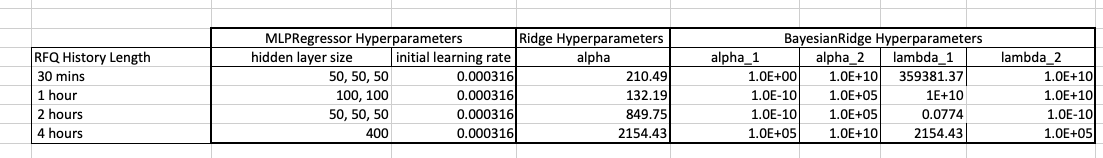
\includegraphics[width=1.2\linewidth]{./figures/Ch4_best_hyperprms_c}
    \resizebox{\linewidth}{!}{\begin{tabular}{lcccccccccc}
        \toprule
        &&
        \multicolumn{2}{c}{MLP Regressor} &&
        \multicolumn{1}{c}{Ridge} &&
        \multicolumn{4}{c}{Bayesian Ridge} \\
        &&
        \multicolumn{2}{c}{Hyperparameters} &&
        \multicolumn{1}{c}{Hyperparameters} &&
        \multicolumn{4}{c}{Hyperparameters} \\
        \cmidrule{3-4}\cmidrule{6-6}\cmidrule{8-11}
                                   & & hidden     & initial  & &         & &             &            &             &             \\
                                   & & layer      & learning & &         & &             &            &             &             \\
        RFQ HistoryLength          & & size       & rate     & & alpha   & & alpha$_1$   & alpha$_2$  & lambda$_1$  & lambda$_2$  \\
        \midrule
        Count and Notional 30~mins & & 100, 100   & 0.000316 & &  335.16 & & \num{1e-10} & \num{1e10} & 359381.37   & \num{1e10}  \\
        Count and Notional 1~hour  & & 50, 50, 50 & 0.000316 & &  335.16 & & \num{1e0}   & \num{1e5}  & 359381.37   & \num{1e5}  \\
        Count and Notional 2~hours & & 100, 100   & 0.000316 & & 1353.05 & & \num{1e-10} & \num{1e5}  &  12.92      & \num{1e0} \\
        Count and Notional 4~hours & & 100, 100   & 0.000316 & & 2154.43 & & \num{1e0}   & \num{1e10} & \num{1e-10} & \num{1e-5}   \\
        \bottomrule
    \end{tabular}}
\end{table}

\clearpage
\begin{figure}[!ht]\centering
    \begin{subfigure}[t]{.47\linewidth}\centering
        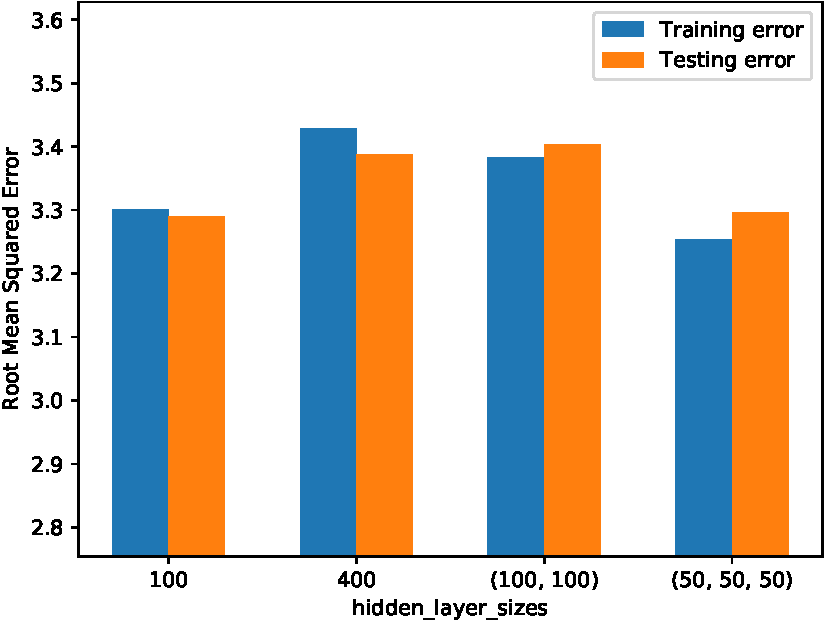
\includegraphics[width=0.9\linewidth]{./figures/AplotA1.pdf}
        \caption{RMS error vs.~architecture for 1~hour count history}\label{AppAplotA1}
    \end{subfigure}\hfill%
    \begin{subfigure}[t]{.47\linewidth}\centering
        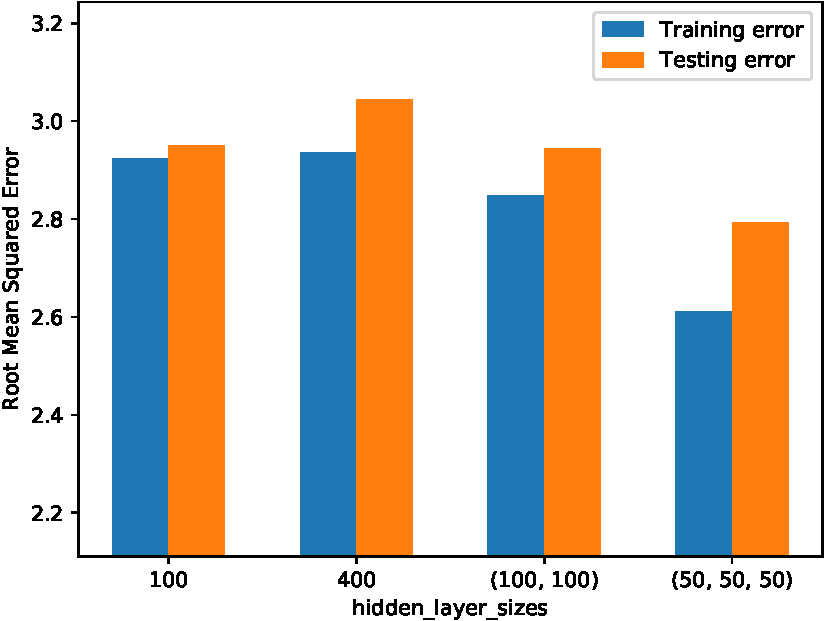
\includegraphics[width=0.9\linewidth]{./figures/AplotA2.pdf}
        \caption{RMS error vs.~architecture for 2~hours count history}\label{AppAplotA2}
    \end{subfigure}\\[5pt]
    \begin{subfigure}[t]{.47\linewidth}\centering
        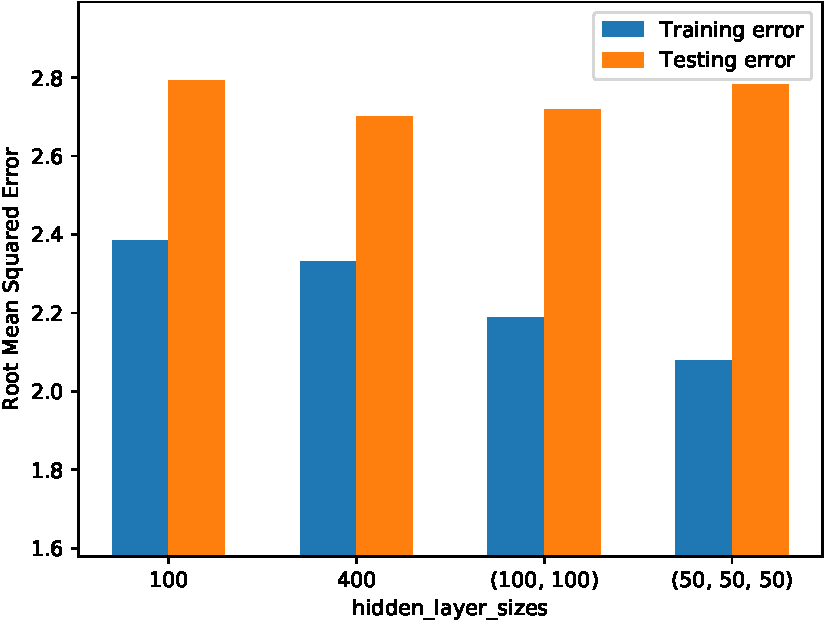
\includegraphics[width=0.9\linewidth]{./figures/AplotA3.pdf}
        \caption{RMS error vs.~architecture for 4~hours count history}\label{AppAplotA3}
    \end{subfigure}\hfill%
    \begin{subfigure}[t]{.47\linewidth}\centering
        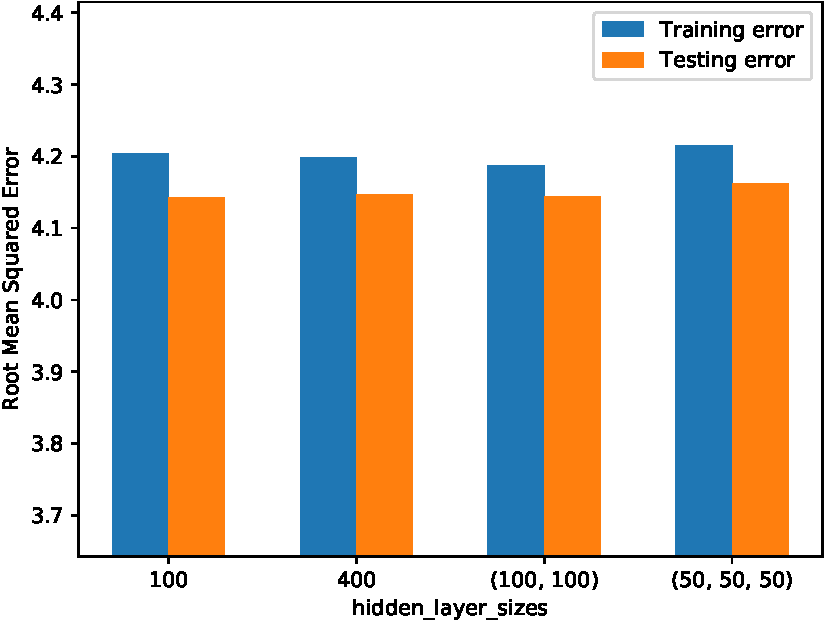
\includegraphics[width=0.9\linewidth]{./figures/AplotA4.pdf}
        \caption{RMS error vs.~architecture for 30~mins count history}\label{AppAplotA4}
    \end{subfigure}\\[5pt]
    \begin{subfigure}[t]{.47\linewidth}\centering
        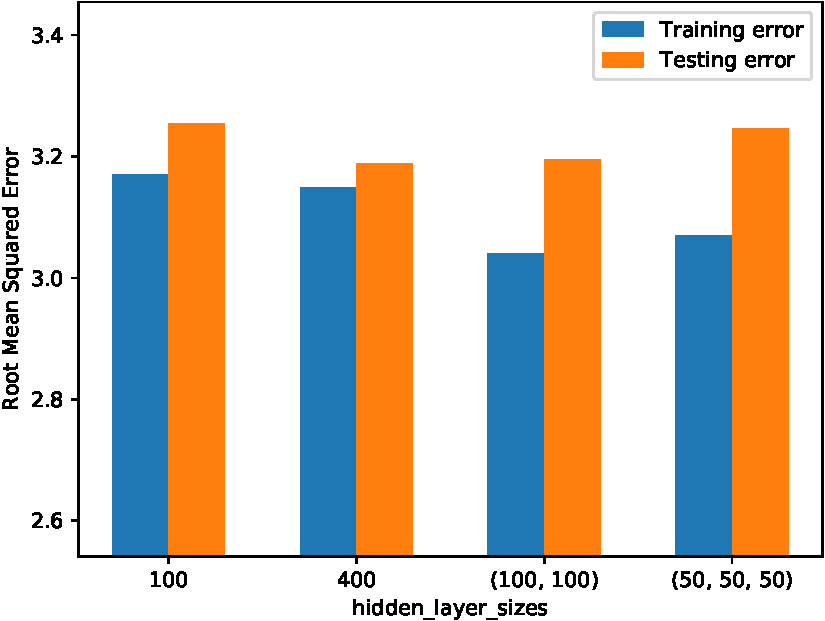
\includegraphics[width=0.9\linewidth]{./figures/AplotA5.pdf}
        \caption{RMS error vs.~architecture for 1~hours count and notional history}\label{AppAplotA5}
    \end{subfigure}\hfill%
    \begin{subfigure}[t]{.47\linewidth}\centering
        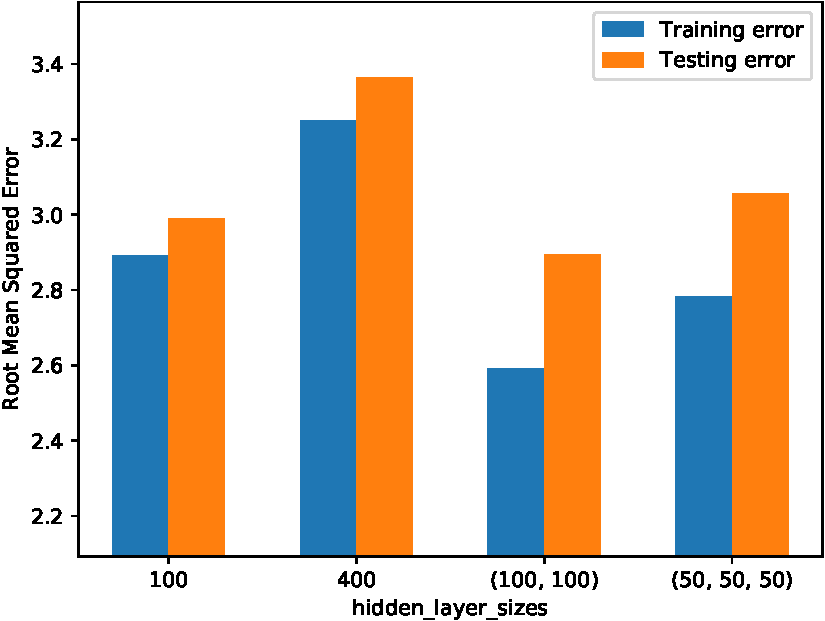
\includegraphics[width=0.9\linewidth]{./figures/AplotA6.pdf}
        \caption{RMS error vs.~architecture for 2~hours count and notional history}\label{AppAplotA6}
    \end{subfigure}\\[5pt]
    \begin{subfigure}[t]{.47\linewidth}\centering
        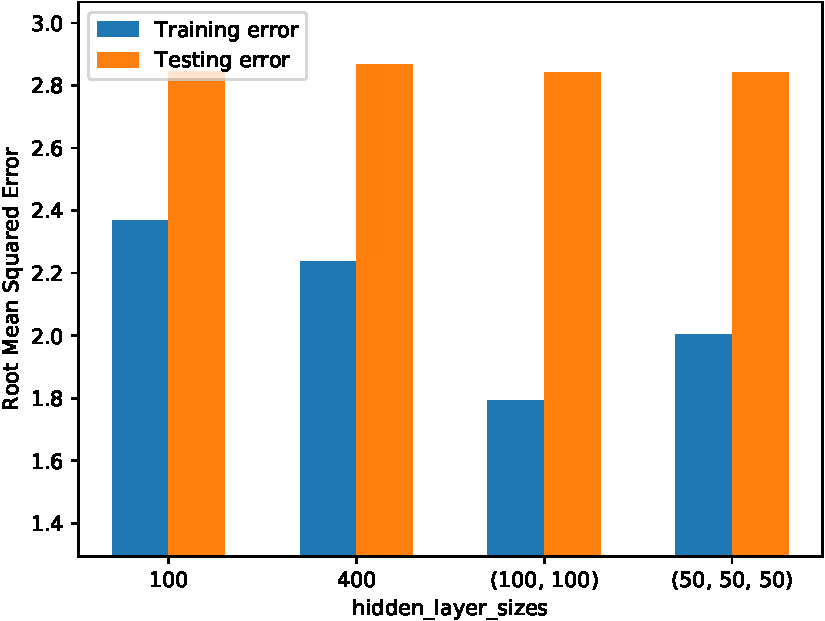
\includegraphics[width=0.9\linewidth]{./figures/AplotA7.pdf}
        \caption{RMS error vs.~architecture for 4~hours count and notional history}\label{AppAplotA7}
    \end{subfigure}\hfill%
    \begin{subfigure}[t]{.47\linewidth}\centering
        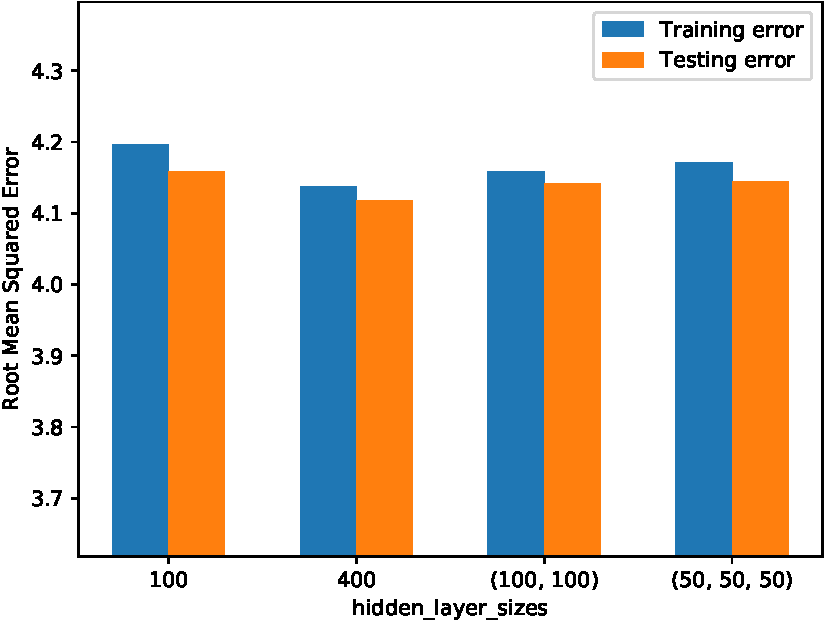
\includegraphics[width=0.9\linewidth]{./figures/AplotA8.pdf}
        \caption{RMS error vs.~architecture for 30~mins count and notional history}\label{AppAplotA8}
    \end{subfigure}
    \caption{Experiment 1 -- MLPRegressor RMS error vs.~network architecture plots}\label{App:Exp1_plots1}
\end{figure}

\clearpage
\begin{figure}[!ht]\centering
    \begin{subfigure}[t]{.47\linewidth}\centering
        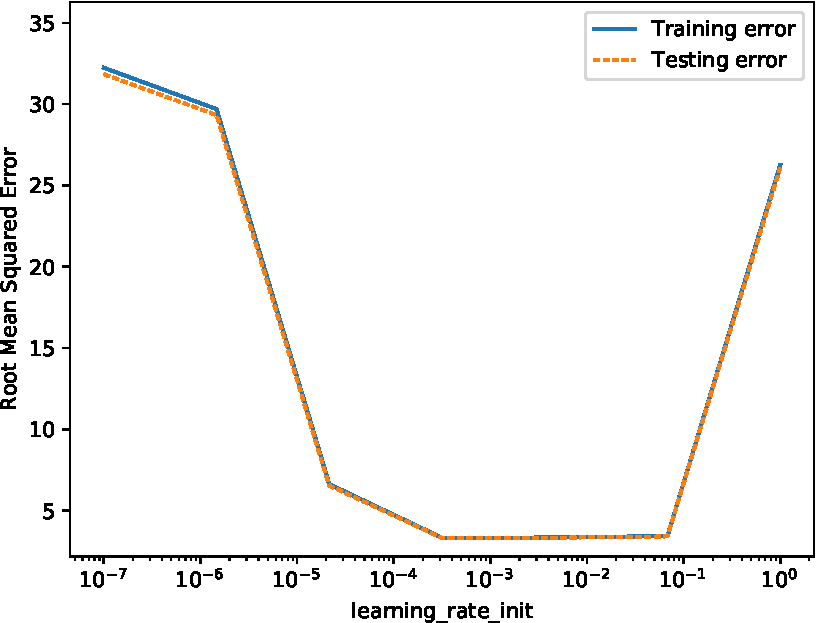
\includegraphics[width=0.9\linewidth]{./figures/AplotB1.pdf}
        \caption{RMS error vs.~initial learning rate for 1~hour count history}\label{AppAplotB1}
    \end{subfigure}\hfill%
    \begin{subfigure}[t]{.47\linewidth}\centering
        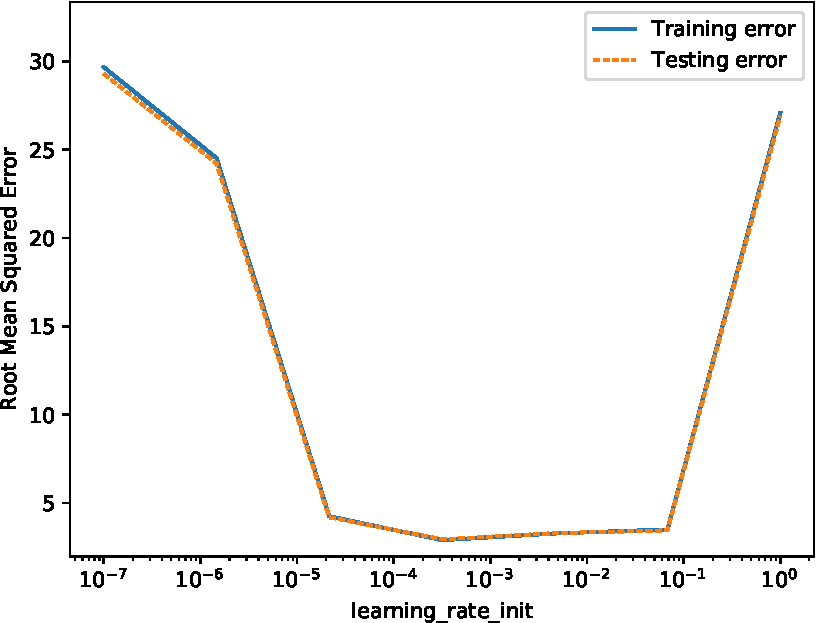
\includegraphics[width=0.9\linewidth]{./figures/AplotB2.pdf}
        \caption{RMS error vs.~initial learning rate for 2~hours count history}\label{AppAplotB2}
    \end{subfigure}\\[5pt]
    \begin{subfigure}[t]{.47\linewidth}\centering
        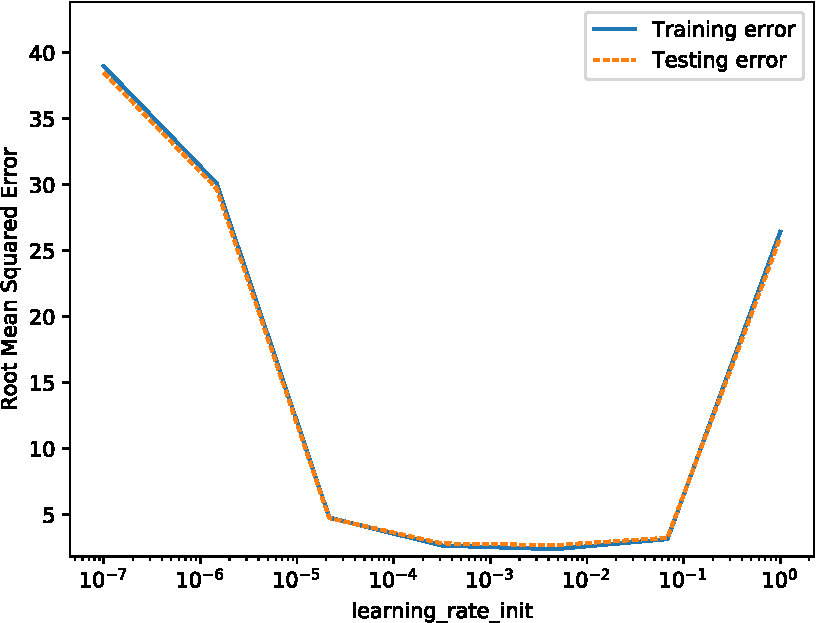
\includegraphics[width=0.9\linewidth]{./figures/AplotB3.pdf}
        \caption{RMS error vs.~initial learning rate for 4~hours count history}\label{AppAplotB3}
    \end{subfigure}\hfill%
    \begin{subfigure}[t]{.47\linewidth}\centering
        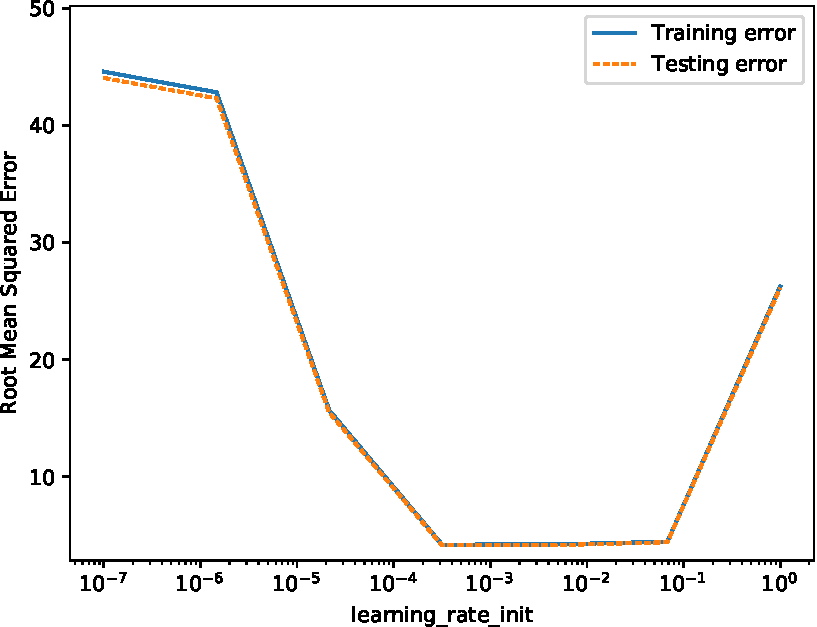
\includegraphics[width=0.9\linewidth]{./figures/AplotB4.pdf}
        \caption{RMS error vs.~initial learning rate for 30~mins count history}\label{AppAplotB4}
    \end{subfigure}\\[5pt]
    \begin{subfigure}[t]{.47\linewidth}\centering
        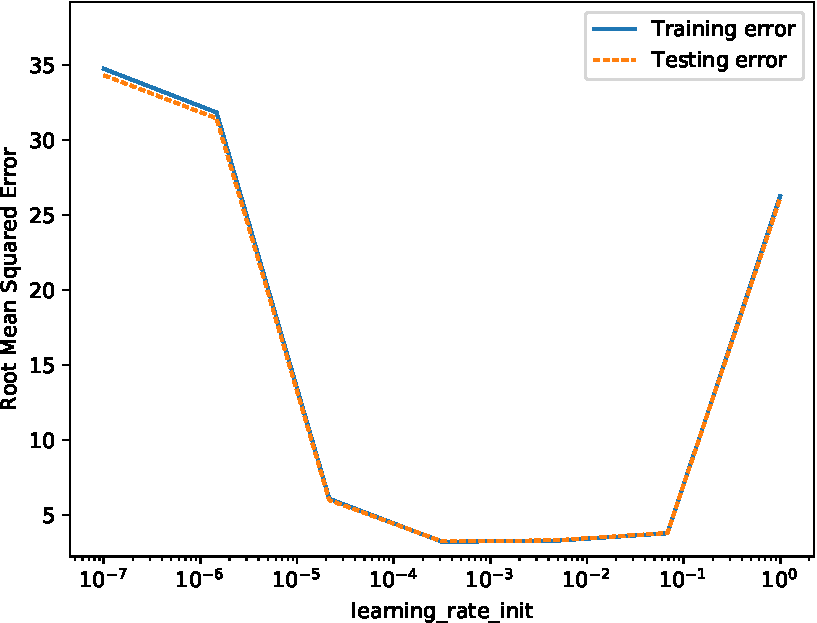
\includegraphics[width=0.9\linewidth]{./figures/AplotB5.pdf}
        \caption{RMS error vs.~initial learning rate for 2~hours count and notional history}\label{AppAplotB5}
    \end{subfigure}\hfill%
    \begin{subfigure}[t]{.47\linewidth}\centering
        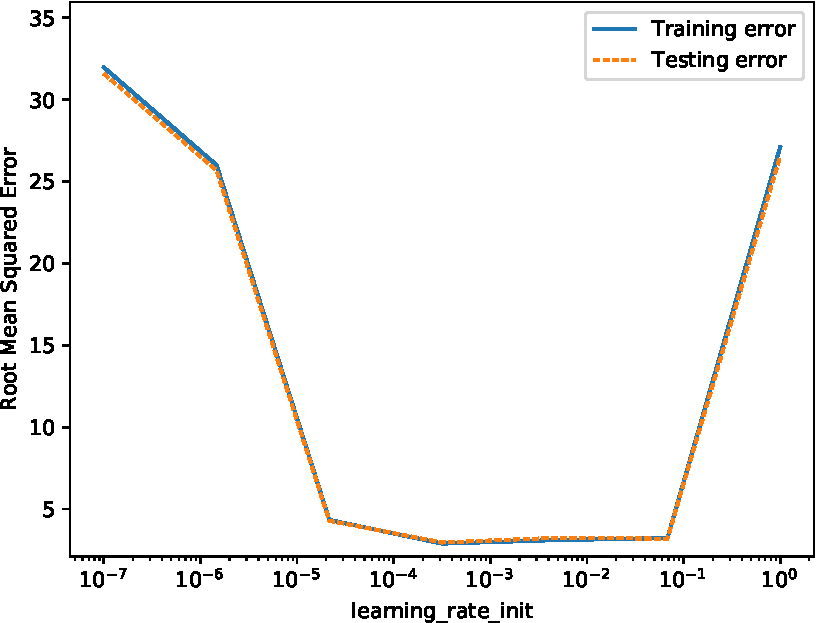
\includegraphics[width=0.9\linewidth]{./figures/AplotB6.pdf}
        \caption{RMS error vs.~initial learning rate for 2~hours count and notional history}\label{AppAplotB6}
    \end{subfigure}\\[5pt]
    \begin{subfigure}[t]{.47\linewidth}\centering
        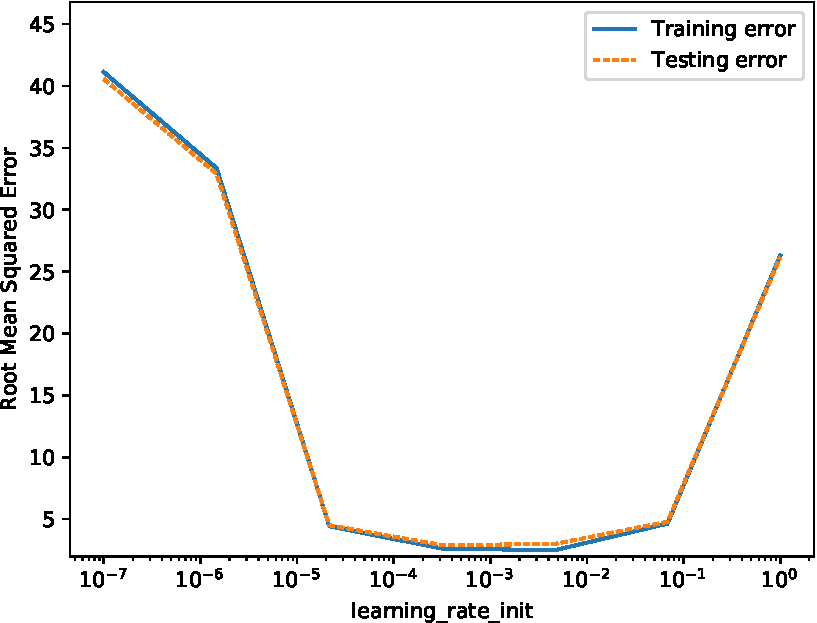
\includegraphics[width=0.9\linewidth]{./figures/AplotB7.pdf}
        \caption{RMS error vs.~initial learning rate for 4~hours count and notional history}\label{AppAplotB7}
    \end{subfigure}\hfill%
    \begin{subfigure}[t]{.47\linewidth}\centering
        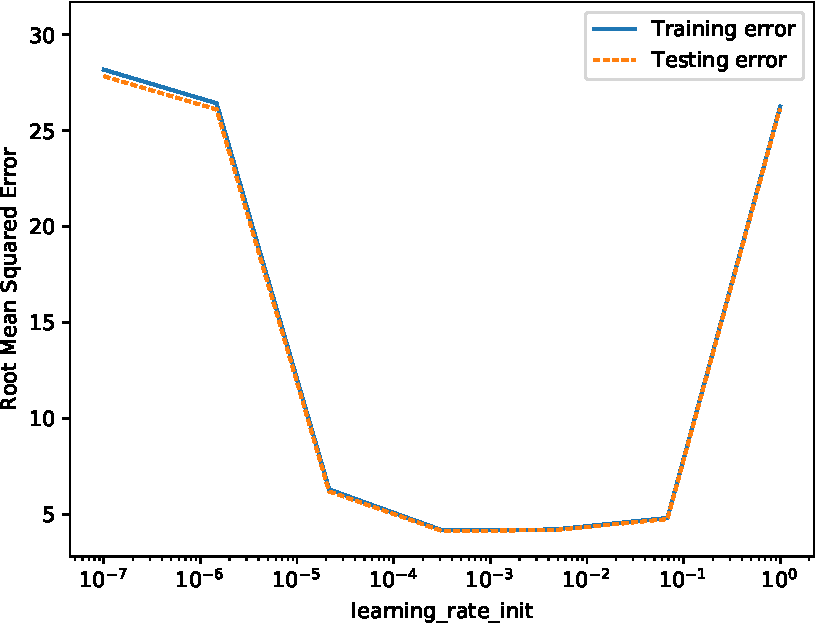
\includegraphics[width=0.9\linewidth]{./figures/AplotB8.pdf}
        \caption{RMS error vs.~initial learning rate for 30~mins count and notional history}\label{AppAplotB8}
    \end{subfigure}
    \caption{Experiment 1 -- MLPRegressor plots of RMS error sensitivity to initial learning rate }\label{App:Exp1_plots2}
\end{figure}

\clearpage
\begin{figure}[!ht]\centering
    \begin{subfigure}[t]{.47\linewidth}\centering
        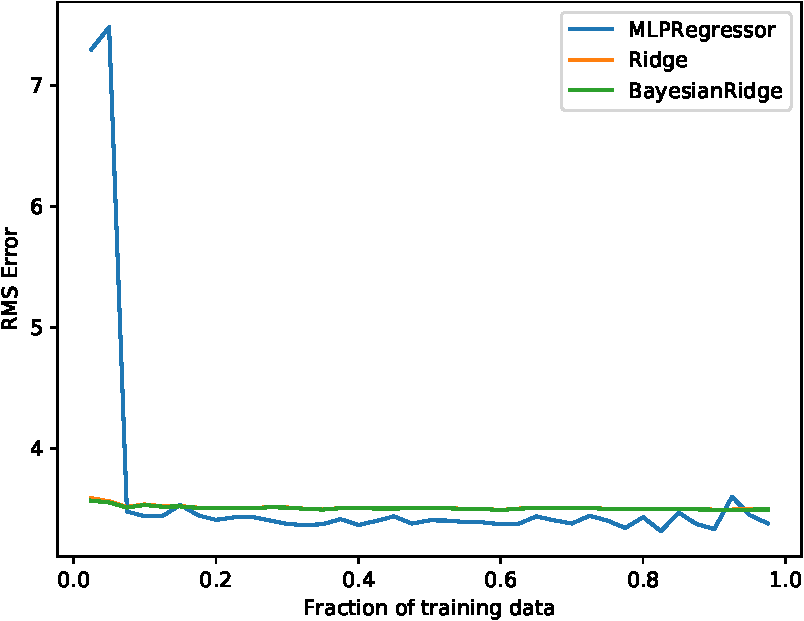
\includegraphics[width=0.9\linewidth]{./figures/AplotC1.pdf}
        \caption{RMS Test error vs.~size of training data for 1~hour count}\label{AppAplotC1}
    \end{subfigure}\hfill%
    \begin{subfigure}[t]{.47\linewidth}\centering
        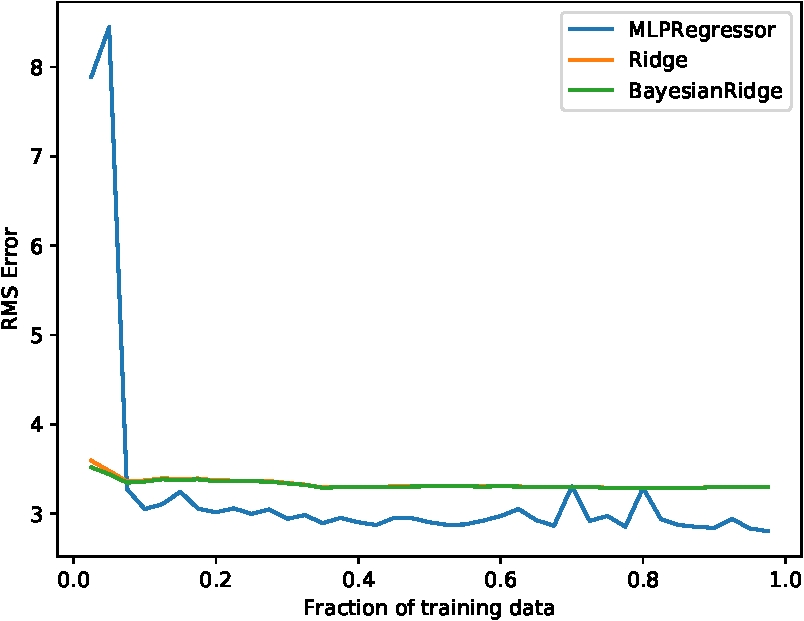
\includegraphics[width=0.9\linewidth]{./figures/AplotC2.pdf}
        \caption{RMS Test error vs.~size of training data for 2~hours count}\label{AppAplotC2}
    \end{subfigure}\\[5pt]
    \begin{subfigure}[t]{.47\linewidth}\centering
        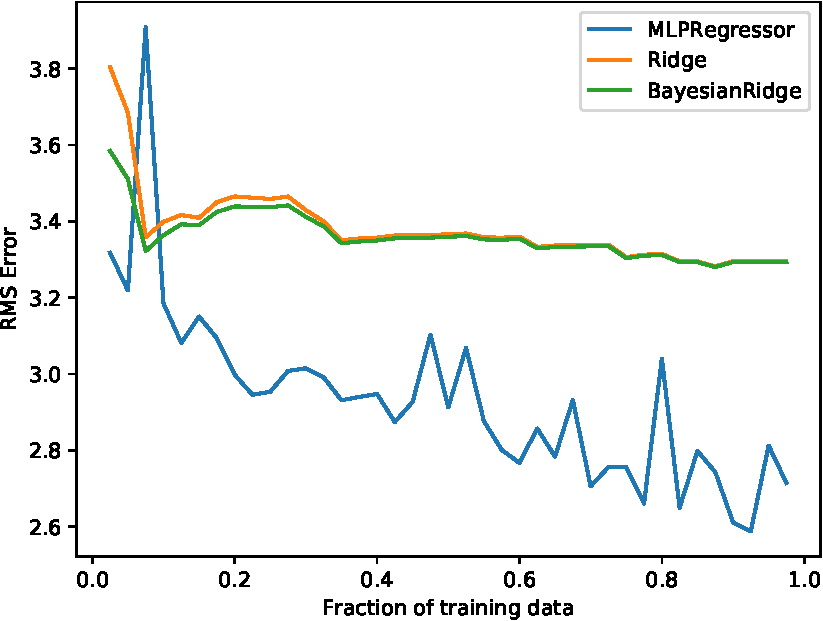
\includegraphics[width=0.9\linewidth]{./figures/AplotC3.pdf}
        \caption{RMS Test error vs.~size of training data for 4~hours count}\label{AppAplotC3}
    \end{subfigure}\hfill%
    \begin{subfigure}[t]{.47\linewidth}\centering
        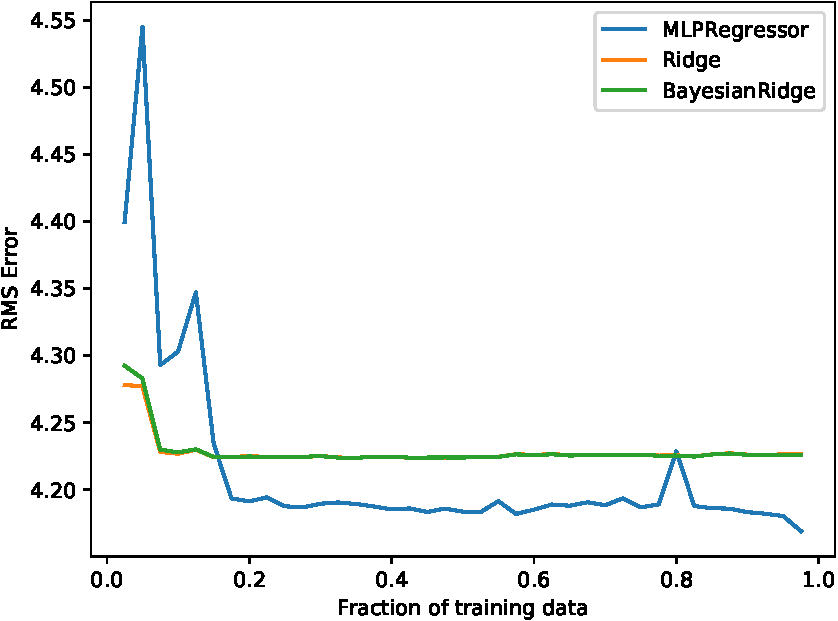
\includegraphics[width=0.9\linewidth]{./figures/AplotC4.pdf}
        \caption{RMS Test error vs.~size of training data for 30~mins count}\label{AppAplotC4}
    \end{subfigure}\\[5pt]
    \begin{subfigure}[t]{.47\linewidth}\centering
        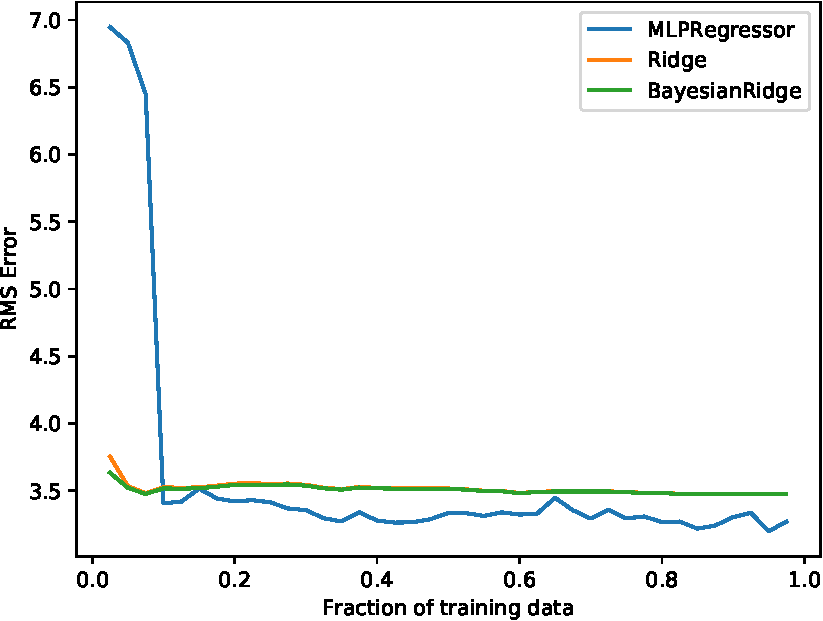
\includegraphics[width=0.9\linewidth]{./figures/AplotC5.pdf}
        \caption{RMS Test error vs.~size of training data for 1~hour count and notional}\label{AppAplotC5}
    \end{subfigure}\hfill%
    \begin{subfigure}[t]{.47\linewidth}\centering
        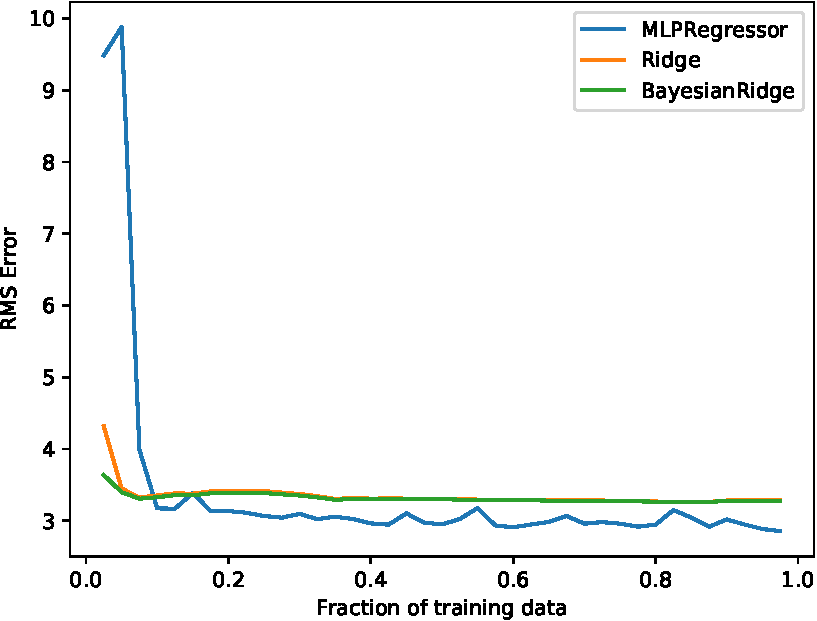
\includegraphics[width=0.9\linewidth]{./figures/AplotC6.pdf}
        \caption{RMS Test error vs.~size of training data for 2~hours count and notional}\label{AppAplotC6}
    \end{subfigure}\\[5pt]
    \begin{subfigure}[t]{.47\linewidth}\centering
        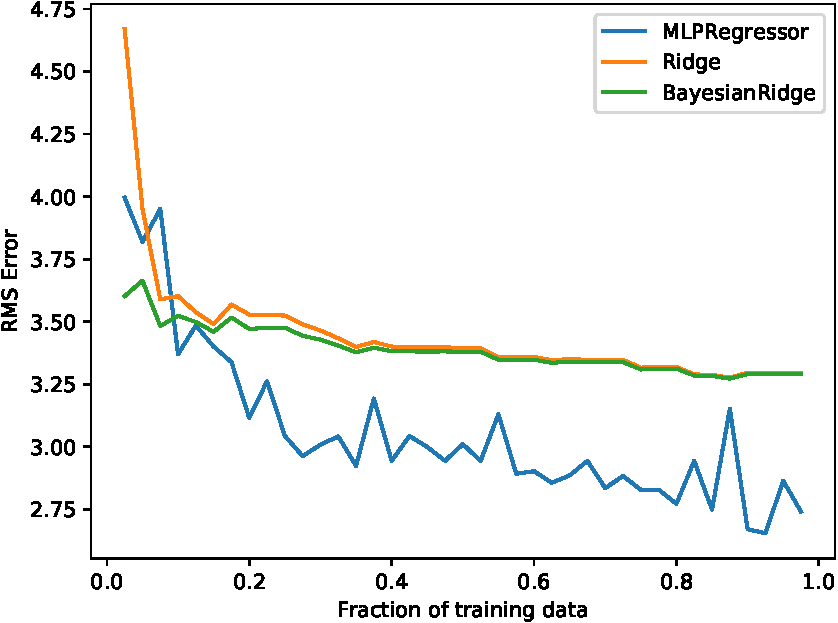
\includegraphics[width=0.9\linewidth]{./figures/AplotC7.pdf}
        \caption{RMS Test error vs.~size of training data for 4~hours count and notional}\label{AppAplotC7}
    \end{subfigure}\hfill%
    \begin{subfigure}[t]{.47\linewidth}\centering
        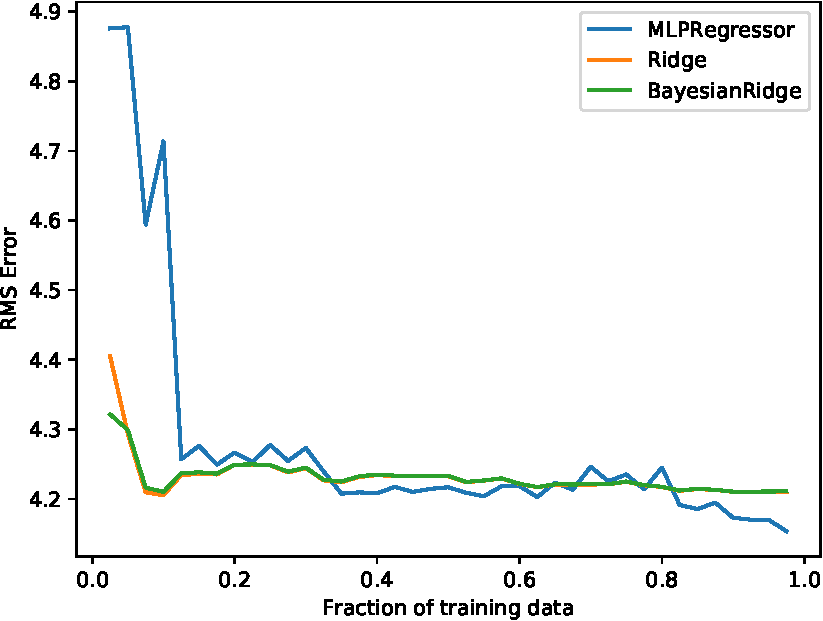
\includegraphics[width=0.9\linewidth]{./figures/AplotC8.pdf}
        \caption{RMS Test error vs.~size of training data for 30~mins count and notional}\label{AppAplotC8}
    \end{subfigure}
        \caption{Experiment 1 -- RMS Test error for each model vs.~size of training data}\label{App:Exp1_plots3}
\end{figure}

\clearpage
\begin{figure}[!t]\centering
    \begin{subfigure}[t]{.475\linewidth}\centering
        \includegraphics[width=1\linewidth]{./figures/BayesianRidgelambda14hr.pdf}
        \caption{RSM error sensitivity vs.~lambda$_1$ hyperparameters for Bayesian Ridge }\label{App:A4a}
    \end{subfigure}\hfill%
    \begin{subfigure}[t]{.475\linewidth}\centering
        \includegraphics[width=1\linewidth]{./figures/Ridgealpha4hr.pdf}
        \caption{RSM error sensitivity vs.~alpha hyperparameters for Ridge}\label{App:A4b}
    \end{subfigure}
        \caption{RSM error sensitivity vs.~hyperparameters for Bayesian Ridge and Ridge}\label{App:A4}
\end{figure}
\vfill
\strut